\chapter{IoT, Robotics \& Safety as a Design Obligation}
\label{ch9}

\paragraph{Where this fits.}
This chapter operates at Stage~3 (Development) of the Stage-Gate model.
Security and physical-safety requirements not designed in at this stage will
surface as failures at Gate~4 (Testing \& Validation), where every retrofit
costs more time, more money, and more risk than the original design decision
would have.
A security flaw discovered during a field test does not cost one library swap;
it costs a firmware re-architecture, a re-flash campaign, and a delay that may
miss the project deadline.
A prototype moving part without a hardware emergency stop does not fail quietly;
it fails dangerously.

\paragraph{Learning Objectives.}
After completing this chapter you will be able to:
\begin{enumerate}
  \item Identify the three IoT attack surfaces and specify at least one security
        control for each.
  \item Compute average current $I_{\text{avg}}$ and battery life $t_{\text{life}}$
        for a duty-cycled IoT device.
  \item Identify the three required physical-safety features for a moving robotic
        prototype: e-stop, guarding, and fail-safe state.
  \item Compute the mechanical safety factor $\mathrm{SF}$ for a load-bearing
        element and assess whether $\mathrm{SF} \geq 2$ is satisfied.
\end{enumerate}

Chapter~8 delivered a working firmware prototype built with AI-assisted tooling
inside Stage~3.
That left open a second set of Stage~3 obligations: the security, power, and
physical-safety requirements that the hardware itself carries --- regardless of
what tools were used to design it.
This chapter closes that gap.

% ─────────────────────────────────────────────────────────────────────────────
\section{IoT Security by Design}
\label{sec:ch9-security}
% ─────────────────────────────────────────────────────────────────────────────

\textbf{Security by design}\index{security by design} means treating encryption,
authentication, and secure communication as first-class design requirements, not
optional enhancements added after the hardware is built and running.

The cost-of-change principle from Chapter~3 applies directly: the three security
properties below must be designed in, not added after.

\textbf{Encryption}\index{encryption} ensures that data in transit cannot be read
or modified by a third party.
For an MQTT sorter node communicating over Wi-Fi, this means TLS~1.2 or TLS~1.3
between the device and the broker.
Encryption without authentication is incomplete: an attacker who cannot read your
messages can still inject their own if the broker accepts unauthenticated
connections.

\textbf{Authentication}\index{authentication} ensures that only legitimate devices
and users can connect to your system.
At minimum, each device must present a unique credential --- a per-device username
and password, or a client certificate --- that the broker can verify and revoke
independently of every other device.
Shared credentials, such as a single ``device'' account used by all nodes, mean
that compromising one device compromises every device on the network.

\textbf{Secure update}\index{secure firmware update} closes the lifecycle loop.
Firmware that cannot be updated securely in the field is firmware that will run
outdated cryptographic libraries indefinitely.
Signing firmware images with a private key and verifying the signature on the
device before flashing is the minimum acceptable posture for any deployed IoT
prototype.

\paragraph{In Practice.}
An IoT prototype shipped with default MQTT broker credentials (``admin'' /
``password'').
Within 48~hours of deployment, a network scanner found the open broker and began
injecting spurious sort commands into the conveyor system.
The fix --- per-device credentials and TLS --- took two days to implement after
the fact.
At design time, the same change would have taken twenty minutes.

% ─────────────────────────────────────────────────────────────────────────────
\section{Attack Surfaces}
\label{sec:ch9-attack}
% ─────────────────────────────────────────────────────────────────────────────

Every IoT system has three distinct \textbf{attack surfaces}\index{attack surface}:
the layer at which an adversary can attempt to gain unauthorised access or
cause harm.
Understanding the surfaces helps you assign a control to each one at design time
rather than discovering them during a security audit.

Figure~\ref{fig:ch9-attack} maps each layer to its principal threats.

\begin{figure}[htbp]
  \centering
  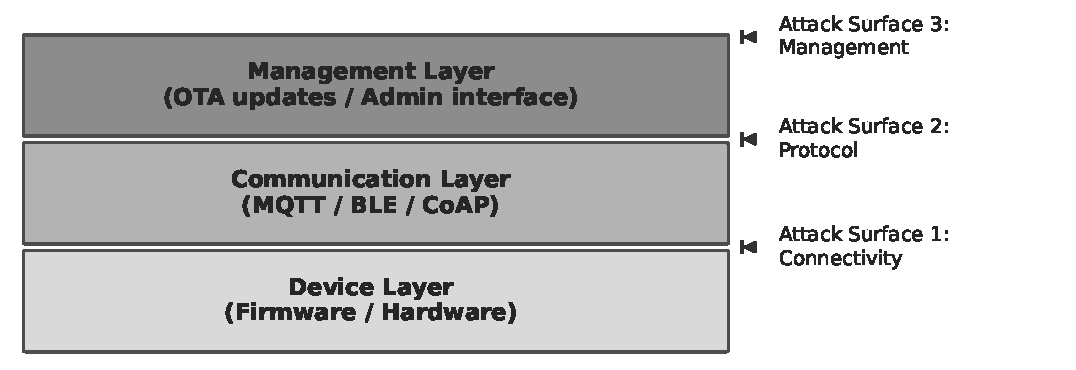
\includegraphics[width=0.85\textwidth]{images/fig_01_attack_surface}
  \caption{Layered IoT architecture for the MQTT sorter node.
           The connectivity layer (Wi-Fi/Ethernet), the communication layer
           (MQTT broker and topics), and the management layer (OTA update
           and admin interface) each carry a distinct attack surface requiring
           its own security control.}
  \label{fig:ch9-attack}
\end{figure}

\subsection{Connectivity Layer}
\label{sec:ch9-attack-connectivity}

The \textbf{connectivity layer}\index{connectivity layer} is the physical and
link-layer network: Wi-Fi, Ethernet, or a cellular radio.
Threats here include passive eavesdropping on unencrypted traffic, man-in-the-middle
insertion, and denial-of-service through radio jamming or TCP flooding.

Apply network-layer encryption (WPA3 for Wi-Fi; VPN or private APN for
cellular) and restrict the device to a dedicated IoT VLAN that has no route to
general office or campus infrastructure.
For the running-example sorter node, the MQTT broker should be reachable only from
the IoT VLAN, not from a shared student network.

\subsection{Communication Layer}
\label{sec:ch9-attack-communication}

The \textbf{communication layer}\index{communication layer} is the application
protocol: MQTT topics, CoAP resources, or BLE GATT characteristics.
Threats here include topic spoofing (an attacker publishes false sensor readings or
spurious actuator commands), topic enumeration (an attacker subscribes to
\texttt{\#} and reads every message), and replay attacks (a captured command is
re-sent later).

Authenticate every publisher and subscriber at the broker using per-device
credentials; use topic-level access control lists (ACLs) so that a sensor node can
publish to its own telemetry topic but cannot publish to the actuator command topic;
include a message timestamp or sequence number to detect replays.

\subsection{Management Layer}
\label{sec:ch9-attack-management}

The \textbf{management layer}\index{management layer} is the interface used to
update firmware and configure the device: an OTA update server, a web dashboard,
an SSH port, or a JTAG adapter left enabled in production firmware.

Threats here are the most severe because compromising the management layer gives
an attacker the ability to re-flash every device.
Disable all debug interfaces in release builds; sign firmware images; use
mutual TLS for OTA update channels; change all default admin credentials before
first deployment; enforce multi-factor authentication on the cloud dashboard.

\paragraph{Common Pitfalls.}
``Add security later'' is the most expensive four-word sentence in embedded
development.
Retrofitting TLS onto an MQTT stack that was built without it requires restructuring
the firmware state machine --- the connection, subscription, publish, and reconnect
logic all carry TLS context --- not just swapping a library call.
The second pitfall is shipping default credentials in production firmware.
Every device with identical credentials is a single point of compromise: one
leaked password grants access to the entire deployed fleet.

% ─────────────────────────────────────────────────────────────────────────────
\section{Privacy and Data Obligations}
\label{sec:ch9-privacy}
% ─────────────────────────────────────────────────────────────────────────────

Sensor data is not automatically neutral.
Certain categories of data collected by an IoT device trigger legal and ethical
obligations that your design must accommodate from the start.

\textbf{Personal data}\index{personal data} is any information that can identify a
natural person, directly or indirectly.
A CO$_2$ sensor reporting aggregate room occupancy is not personal data; a badge
reader logging individual entry times is.
Under Qu\'{e}bec Law~25 (Loi~25) and the federal PIPEDA, collecting personal data
requires a stated purpose, user consent, and documented retention limits.
If your IoT device collects personal data, you must specify those elements before
the device is deployed.

\textbf{Location data}\index{location data} is a subcategory that receives
heightened scrutiny because it reveals movement patterns over time.
A GPS tag on a delivery robot that reports position continuously creates a
persistent location history.
Design controls include anonymisation (report zone, not coordinates), aggregation
(report 10-minute averages, not 1-second fixes), and retention limits (purge data
older than 30~days).

\textbf{Biometric data}\index{biometric data} --- fingerprint templates, facial
recognition embeddings, voice prints --- is treated as sensitive in virtually
every jurisdiction.
If a prototype uses a camera for person detection, you must assess whether the
processing constitutes biometric identification and, if so, obtain explicit consent
and provide a technical architecture that does not transmit raw biometric templates
over a network.

The practical rule at Stage~3 is: for each sensor on your device, ask whether the
data it produces could identify a person or reveal their behaviour.
If yes, document the legal basis for collection, the purpose limitation, and the
retention policy in your design records before Gate~3.

% ─────────────────────────────────────────────────────────────────────────────
\section{Protocol Selection}
\label{sec:ch9-protocol}
% ─────────────────────────────────────────────────────────────────────────────

Choosing a communication protocol is simultaneously a security decision, a power
decision, and an interoperability decision; each of the three protocols used at
prototype scale --- MQTT, CoAP, and BLE --- carries a distinct security posture
and power profile requiring its own design controls.

\subsection{MQTT}
\label{sec:ch9-protocol-mqtt}

\textbf{MQTT}\index{MQTT} (Message Queuing Telemetry Transport) is a
publish-subscribe protocol designed for constrained devices on unreliable networks.
It is TCP-based, which means it carries the overhead of a persistent connection but
provides reliable, ordered delivery.
For the running-example sorter node, MQTT is the protocol of record.

Mandatory security posture for MQTT in a prototype:
\begin{itemize}
  \item Use TLS~1.2 or TLS~1.3 between every client and the broker.
        Plain-text MQTT on port~1883 is not acceptable on any network reachable
        from the internet.
  \item Use an \textbf{authenticated broker}\index{authenticated broker}: the
        broker must require a username and password (or client certificate) before
        accepting a connection.
  \item Issue \textbf{per-device credentials}\index{per-device credentials}:
        each node has its own username/password pair so that a compromised node
        can be revoked without affecting any other device.
  \item Define topic ACLs so that sensor nodes cannot publish to actuator command
        topics.
\end{itemize}

\subsection{CoAP}
\label{sec:ch9-protocol-coap}

\textbf{CoAP}\index{CoAP} (Constrained Application Protocol) is a
request-response protocol modelled on HTTP but designed for UDP transport and
very small code footprints.
It is appropriate when the device cannot maintain a persistent TCP connection or
when a RESTful resource model fits the application better than a topic hierarchy.

Security posture: use DTLS (Datagram TLS) to secure CoAP traffic.
Plain-text CoAP has no confidentiality or integrity protection.
DTLS adds handshake overhead to each session, but pre-shared key (PSK) mode keeps
the footprint manageable on constrained microcontrollers.

\subsection{BLE}
\label{sec:ch9-protocol-ble}

\textbf{BLE}\index{BLE} (Bluetooth Low Energy) is a short-range, low-power
protocol suited to wearables, beacons, and devices that communicate with a
nearby gateway or smartphone.
Its power consumption advantage over Wi-Fi is significant: a BLE advertisement
at 1~dBm typically costs less than 10~mA for a few milliseconds, while a Wi-Fi
association sequence can draw 100--200~mA for hundreds of milliseconds.

Security posture: use \textbf{LE Secure Connections}\index{LE Secure Connections}
(introduced in Bluetooth~4.2), which uses Elliptic Curve Diffie-Hellman for key
exchange.
Legacy ``Just Works'' pairing provides no meaningful security against passive
eavesdropping; avoid it in any design that transmits data of value.

The trade-off summary: MQTT over TLS is the right choice for the sorter node
because the broker provides centralised logging, topic ACLs, and a dashboard
integration point.
BLE would be appropriate if the node were battery-powered and within 10~m of a
gateway.
CoAP is appropriate for constrained nodes that cannot sustain a TCP connection.

% ─────────────────────────────────────────────────────────────────────────────
\section{Power and Battery Budgeting}
\label{sec:ch9-power}
% ─────────────────────────────────────────────────────────────────────────────

Battery-powered IoT nodes operate in a \textbf{duty cycle}\index{duty cycle}:
they wake, perform a measurement and a transmission, then return to a deep-sleep
mode that draws a fraction of the active current.
The duty cycle $D$ is the fraction of time the device spends in its active state.

\subsection{Average Current}
\label{sec:ch9-power-iavg}

Because the device spends most of its time asleep, the battery sees a time-weighted
average current that is much lower than the active current.
The \textbf{average current}\index{average current} $I_{\text{avg}}$ is:

\begin{equation}\label{eq:ch9-iavg}
  I_{\text{avg}} = D \cdot I_{\text{active}} + (1-D) \cdot I_{\text{sleep}}
\end{equation}

where $I_{\text{active}}$ is the current drawn during the active interval,
$I_{\text{sleep}}$ is the current drawn during the sleep interval, and $D$ is the
duty cycle (dimensionless, $0 < D < 1$).

At low duty cycles --- say, $D = 0.02$ (2\,\%) --- the sleep current often
dominates the average even if it is two or three orders of magnitude smaller than
the active current.
This means that reducing $I_{\text{sleep}}$ by choosing a microcontroller with a
lower deep-sleep current may improve battery life more than reducing $I_{\text{active}}$.

\subsection{Battery Life}
\label{sec:ch9-power-tlife}

Given $I_{\text{avg}}$ and a battery capacity $C_{\text{batt}}$ (in mAh), the
estimated \textbf{battery life}\index{battery life} $t_{\text{life}}$ is:

\begin{equation}\label{eq:ch9-tlife}
  t_{\text{life}} = \frac{C_{\text{batt}}}{I_{\text{avg}}}
\end{equation}

This is an idealised estimate.
Real battery capacity degrades with temperature, discharge rate, and age; a
practical design should target $t_{\text{life}}$ at least 20\,\% above the
specification to account for these effects.

Figure~\ref{fig:ch9-power} shows the current profile for a duty-cycled node,
with $I_{\text{avg}}$ marked as the equivalent constant-current drain.

\begin{figure}[htbp]
  \centering
  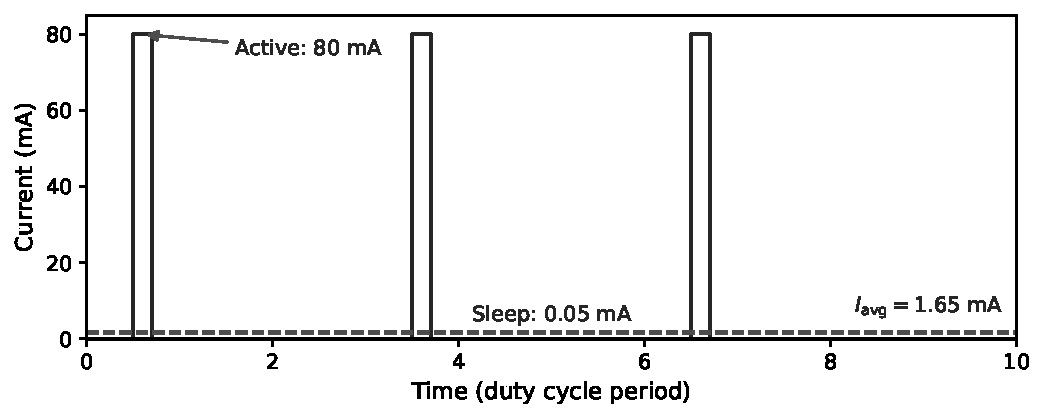
\includegraphics[width=0.85\textwidth]{images/fig_02_power_budget}
  \caption{Duty-cycled current profile for an MQTT sensor node.
           Narrow active pulses (drawing $I_{\text{active}}$) are separated by
           long sleep intervals (drawing $I_{\text{sleep}}$).
           The dashed horizontal line marks $I_{\text{avg}}$, the constant
           current that would drain the battery in the same time.
           At $D = 2\,\%$, the sleep interval dominates the average.}
  \label{fig:ch9-power}
\end{figure}

\subsection{Worked Example --- Power Budget}
\label{sec:ch9-power-worked}

The running-example MQTT sorter node has the following parameters:
$I_{\text{active}} = 80$~mA, $I_{\text{sleep}} = 0.05$~mA, $D = 0.02$
(the node wakes every 10~s for a 200~ms measurement-and-publish cycle),
$C_{\text{batt}} = 2000$~mAh.

\textbf{Step~1: Compute $I_{\text{avg}}$.}

Using Equation~\ref{eq:ch9-iavg}:
\[
  I_{\text{avg}} = 0.02 \times 80 + 0.98 \times 0.05
                = 1.600 + 0.049
                = 1.649~\text{mA}
\]

\textbf{Step~2: Compute $t_{\text{life}}$.}

Using Equation~\ref{eq:ch9-tlife}:
\[
  t_{\text{life}} = \frac{2000}{1.649} = 1212.9~\text{h} \approx 50.5~\text{days}
\]

\textbf{Step~3: Sensitivity --- halve the duty cycle.}

If the team can reduce the reporting rate so that $D = 0.01$ (one report per
20~s instead of per 10~s):
\[
  I_{\text{avg}}' = 0.01 \times 80 + 0.99 \times 0.05 = 0.800 + 0.0495 = 0.8495~\text{mA}
\]
\[
  t_{\text{life}}' = \frac{2000}{0.8495} \approx 2354~\text{h} \approx 98.1~\text{days}
\]

Halving the duty cycle nearly doubles the battery life (from 50.5~days to
98.1~days).
The improvement is not exactly $2\times$ because the sleep current sets a floor:
as $D \to 0$, $I_{\text{avg}} \to I_{\text{sleep}}$, not zero.
This sensitivity analysis belongs in the power budget table of your design
records.

% ─────────────────────────────────────────────────────────────────────────────
\section{Robotics Physical Safety}
\label{sec:ch9-robot}
% ─────────────────────────────────────────────────────────────────────────────

Any prototype that moves --- a conveyor, a sort gate, a rotating arm, a wheeled
platform --- imposes physical-safety obligations that software alone cannot
satisfy.
Three features are non-negotiable for any moving robotic prototype in this
course, and in professional practice.

Figure~\ref{fig:ch9-robot} identifies all three safety features in the
running-example workspace.

\begin{figure}[htbp]
  \centering
  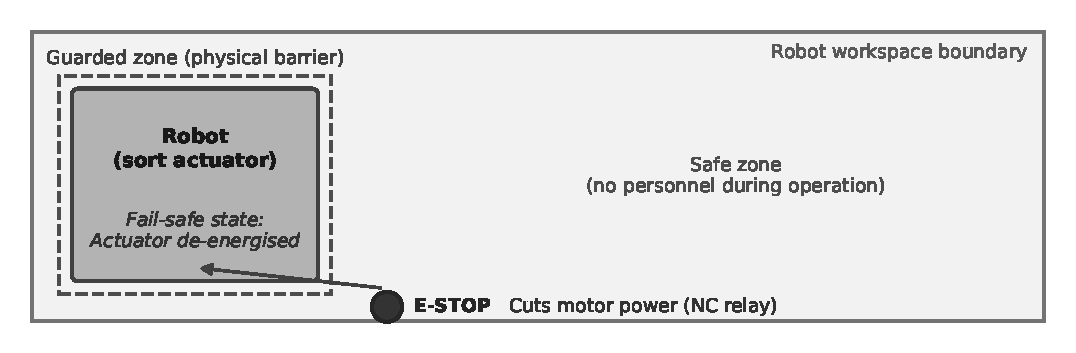
\includegraphics[width=0.85\textwidth]{images/fig_03_robot_safety}
  \caption{Sorter-node robot workspace.
           The exclusion zone (hatched) around the conveyor and sort gate is
           bounded by physical guarding (solid line).
           The e-stop button is positioned in the operator zone, outside the
           guarding, and its normally-closed contact sits in series with the
           motor power rail.
           The fail-safe state (conveyor stopped, gate centred) is the power-off
           default.}
  \label{fig:ch9-robot}
\end{figure}

\subsection{Emergency Stop}
\label{sec:ch9-robot-estop}

An \textbf{emergency stop (e-stop)}\index{emergency stop} is a hardware mechanism
--- not a software function --- that removes power from every actuator when
activated.
The key word is hardware: a normally-closed (NC) relay or contactor in series
with the motor power supply that opens when the e-stop button is pressed or when
the button circuit is broken.

A software e-stop (a flag checked in the main loop, an interrupt service routine
that calls \texttt{motor\_stop()}) does not satisfy this requirement.
If the firmware crashes, the stack overflows, or a runaway interrupt handler locks
the scheduler, the software e-stop cannot execute.
The hardware relay opens regardless of firmware state.

Requirements for the running example:
\begin{itemize}
  \item One NC e-stop button accessible from the operator zone, outside the
        guarding perimeter.
  \item The e-stop contact in series with the 12~V motor supply rail.
  \item Latching action: the system must not restart when the button is released;
        it requires a deliberate reset after the hazard has been cleared.
\end{itemize}

\paragraph{In Practice.}
A robot prototype during a lab test had only a software e-stop.
During a firmware crash, the motor continued running and drove the conveyor belt
into its mechanical end-stop.
The belt was damaged and the test had to be postponed.
A normally-closed hardware relay in the motor power path would have cut power
the instant the crash was detected by the watchdog --- or the moment a person
reached for the e-stop button.

\subsection{Guarding}
\label{sec:ch9-robot-guarding}

\textbf{Guarding}\index{guarding} is a physical barrier that prevents unintended
contact between a person and a moving part.
Guarding is not a ``nice to have''; under Qu\'{e}bec's Act Respecting Occupational
Health and Safety (LSST) and the federal \textit{Canada Labour Code}, any moving
part that presents a hazard must be guarded or rendered inaccessible.

For the bench-scale sorter prototype, acceptable guarding includes:
\begin{itemize}
  \item Acrylic or aluminium side panels along the conveyor belt that prevent
        fingers from reaching the belt, rollers, or sort gate during operation.
  \item An interlocked access panel: if the panel is opened, the interlock opens
        the motor power circuit (the same NC relay used by the e-stop).
  \item A minimum guarding height that prevents reaching over the barrier to the
        nearest pinch point.
\end{itemize}

Guarding must be specified in your design records as a dimensional requirement,
not a verbal intention.
State the material, minimum dimensions, and mounting method.

\subsection{Fail-Safe State}
\label{sec:ch9-robot-failsafe}

A \textbf{fail-safe state}\index{fail-safe state} is the physical state the
system enters when power is removed or a fault is detected.
Designing the fail-safe state requires an explicit decision: what position should
every actuator reach when power is cut?

For the sort gate actuator, the fail-safe state must be the centred (neutral)
position.
This means the actuator spring-returns to centre on power loss, not to the
``sort left'' or ``sort right'' extreme.
For the conveyor motor, the fail-safe state is stopped.
This is achieved by using a spring-return actuator and a motor driver that
de-energises the motor on power loss, not one that holds its last commanded
position.

Use this three-question checklist for each actuator:
\begin{enumerate}
  \item What is the safest physical position on power loss?
  \item Does the mechanism reach that position by gravity, spring return, or
        active braking?
  \item Is the power-off default that position, or does it require a commanded
        move?
\end{enumerate}

If the power-off default is not the safest position, redesign the mechanism or
add a spring return.

\subsection{Force, Speed Limits, and Human-Robot Interaction Zones}
\label{sec:ch9-robot-hri}

Beyond the three required features, professional practice for moving prototypes
includes \textbf{force and speed limits}\index{force limit}\index{speed limit}:
the maximum force an actuator can exert and the maximum speed at which it can
move when a person might be present.

For the bench sorter, define:
\begin{itemize}
  \item A maximum conveyor belt speed (e.g., 0.3~m/s) that limits the kinetic
        energy of items being sorted and reduces the risk of ejection.
  \item A maximum sort-gate actuator force consistent with the SF calculation
        below.
  \item A \textbf{human-robot interaction (HRI) zone}\index{human-robot interaction zone}:
        the area within which a person might reach the moving parts during normal
        operation.
        This zone determines the guarding perimeter.
\end{itemize}

% ─────────────────────────────────────────────────────────────────────────────
\section{Mechanical Safety Factor}
\label{sec:ch9-sf}
% ─────────────────────────────────────────────────────────────────────────────

Every load-bearing element in a moving prototype must be verified against a
minimum \textbf{safety factor}\index{safety factor} $\mathrm{SF}$:

\begin{equation}\label{eq:ch9-sf}
  \mathrm{SF} = \frac{\text{capacity}}{\text{applied load}}
\end{equation}

where capacity is the maximum load the element can sustain before failure (from
material data or simulation) and applied load is the worst-case force the element
will experience in service.
The course minimum is $\mathrm{SF} \geq 2$; this means the element can carry at
least twice the worst-case load before failure.
Any element that fails this criterion requires a redesign before it is installed
in a moving prototype.

\subsection{Worked Example --- Safety Factor}
\label{sec:ch9-sf-worked}

The sort-gate actuator bracket is 3D-printed PLA.
The bracket supports the actuator mass of 0.45~kg.
During a misfire event (the sort gate attempts to move while an item is lodged
in the mechanism), the impact load is estimated at $3\times$ the static weight.

\textbf{Step~1: Compute the applied load.}
\[
  F_{\text{applied}} = 3 \times 0.45~\text{kg} \times 9.81~\text{m/s}^2
                     = 3 \times 4.4145~\text{N} = 13.24~\text{N}
\]

\textbf{Step~2: Compute the capacity.}

From the material specification for this PLA print orientation and infill density,
the tensile strength is 35~MPa.
The bracket cross-section area at the critical section is 2.0~mm$^2$.
\[
  F_{\text{capacity}} = 35~\text{MPa} \times 2.0~\text{mm}^2
                      = 35~\text{N/mm}^2 \times 2.0~\text{mm}^2
                      = 70~\text{N}
\]

\textbf{Step~3: Compute SF.}
\[
  \mathrm{SF} = \frac{70~\text{N}}{13.24~\text{N}} = 5.29
\]

$\mathrm{SF} = 5.29 \geq 2$ --- the bracket passes.

\textbf{Sensitivity check --- reduced cross-section.}

If the design were modified to reduce the cross-section to 0.5~mm$^2$ (to save
material or to route a cable channel through the bracket):
\[
  F_{\text{capacity}}' = 35 \times 0.5 = 17.5~\text{N}
\]
\[
  \mathrm{SF}' = \frac{17.5}{13.24} = 1.32 < 2 \quad \Rightarrow \text{FAILS}
\]

A cross-section of 0.5~mm$^2$ fails the safety criterion.
The bracket must be redesigned --- wider cross-section, different geometry, or
a different material with higher tensile strength --- before it is used.
Record the failing calculation and the redesign rationale in your design records;
Gate~4 reviewers will check that every load-bearing element has a documented SF.

% ─────────────────────────────────────────────────────────────────────────────
\section{EMC, ESD, PPE, and Regulatory Obligations}
\label{sec:ch9-absorbed}
% ─────────────────────────────────────────────────────────────────────────────

Three additional safety disciplines are absorbed into Stage~3 practice: EMC/ESD
design, personal protective equipment (PPE) in the lab, and applicable safety law.

\subsection{EMC and ESD}
\label{sec:ch9-absorbed-emc}

\textbf{Electromagnetic compatibility (EMC)}\index{electromagnetic compatibility}
means that the device neither emits interference above regulated limits nor fails
when exposed to external interference.
For a prototype, the principal EMC obligation at Stage~3 is design hygiene:
decoupling capacitors on every power rail close to each IC, ground planes on the
PCB, and cable routing that minimises loop area.
These are not certification activities; they are design habits that prevent
self-interference and reduce the cost of formal EMC testing later.

\textbf{Electrostatic discharge (ESD)}\index{electrostatic discharge} protection
means that the design can survive the voltage spikes generated by a person
touching the device.
Every I/O pin that is accessible in normal use should have TVS diode protection
or an ESD-rated I/O expander.
For the sorter node, this includes the MQTT status LED pins and the sort-gate
actuator control lines.

\subsection{Lab PPE}
\label{sec:ch9-absorbed-ppe}

\textbf{Personal protective equipment (PPE)}\index{personal protective equipment}
requirements during prototype assembly and testing:
\begin{itemize}
  \item Safety glasses during all power-on testing of circuits above 30~V~DC or
        any circuit with capacitors above 100~$\mu$F.
  \item Anti-static wrist strap when handling bare PCBs or ICs outside of
        anti-static packaging.
  \item No loose clothing or jewellery within the guarded zone of the conveyor
        during any belt-speed test above 0.1~m/s.
\end{itemize}

These are documented in the Vanier College laboratory safety rules and in the
course safety briefing.
They are also design inputs: if the prototype requires testers to work near
exposed moving parts, the guarding design is incomplete.

\subsection{Applicable Safety Law}
\label{sec:ch9-absorbed-law}

Three regulatory frameworks apply to the running example:
\begin{itemize}
  \item \textbf{Qu\'{e}bec LSST} (Act Respecting Occupational Health and Safety):
        requires guarding of all hazardous moving parts and a means of stopping
        the machine in an emergency.
  \item \textbf{Canada Labour Code Part~II}: requires that every employer ensure
        that equipment is safe and that workers are informed of known hazards.
  \item \textbf{IEC~62368-1} (Audio/video, information and communication
        technology equipment --- Safety requirements): the applicable IEC product
        safety standard for the electronic components in the sorter system.
        Compliance is not required for a prototype, but the standard's hazard-based
        safety engineering methodology is the reference model for Stage~3 safety
        decisions.
\end{itemize}

These frameworks do not require certification for a class prototype.
They do require that you are aware of the obligations a product built from this
prototype would carry, and that your design decisions are consistent with meeting
those obligations.

\paragraph{Common Pitfalls.}
Omitting ESD protection on accessible I/O pins.
A single unprotected pin touched during a live test can latch a microcontroller
into an undefined state silently --- no error, no crash, just corrupted peripheral
registers.
TVS diodes cost pennies and are impossible to retrofit onto a finished PCB without
a re-spin.

% ─────────────────────────────────────────────────────────────────────────────
\section{Try It Yourself}
\label{sec:ch9-tiy}
% ─────────────────────────────────────────────────────────────────────────────

A wireless CO$_2$ sensor node has the following parameters:
$I_{\text{active}} = 45$~mA, $I_{\text{sleep}} = 0.08$~mA, $D = 0.05$
(the node wakes for a 3-s measurement cycle every 60~s), $C_{\text{batt}} = 1200$~mAh.
A mounting bracket (aluminium, tensile capacity in this cross-section = 120~N)
supports the sensor mass of 0.30~kg.
The bracket experiences a peak load of $4\times$ the static weight during
installation impact.

\begin{enumerate}
  \item[(a)] Compute $I_{\text{avg}}$ using Equation~\ref{eq:ch9-iavg}.
             Show every arithmetic step.
  \item[(b)] Compute $t_{\text{life}}$ using Equation~\ref{eq:ch9-tlife}.
             Express your answer in hours and in days.
  \item[(c)] The team switches to a lower-power radio that reduces
             $I_{\text{active}}$ to 20~mA while keeping $D = 0.05$.
             Recompute $I_{\text{avg}}$ and $t_{\text{life}}$.
             What is the percentage improvement in battery life compared to part~(b)?
  \item[(d)] Compute the peak applied force in Newtons (use $g = 9.81$~m/s$^2$),
             then compute SF for the bracket using Equation~\ref{eq:ch9-sf}.
             Does the bracket pass the $\mathrm{SF} \geq 2$ criterion?
\end{enumerate}

% ─────────────────────────────────────────────────────────────────────────────
\section{Review Questions}
\label{sec:ch9-review}
% ─────────────────────────────────────────────────────────────────────────────

\begin{enumerate}
  \item[Q1.] \textit{(Conceptual)} Identify the three IoT attack surfaces from
             Section~\ref{sec:ch9-attack}.
             For each, give one security control that applies specifically to
             the running-example MQTT sorter node.

  \item[Q2.] \textit{(Conceptual)} Explain why designing security in at Stage~3
             costs less than retrofitting it at Stage~4.
             Use the cost-of-change principle from Chapter~3 to support your
             argument.
             Your answer should address at least one concrete technical reason
             (not just ``it takes longer'').

  \item[Q3.] \textit{(Applied, calculation)} An IoT sensor has
             $I_{\text{active}} = 120$~mA, $I_{\text{sleep}} = 0.02$~mA,
             $D = 0.03$, $C_{\text{batt}} = 3000$~mAh.
             \begin{enumerate}
               \item[(a)] Compute $I_{\text{avg}}$ using
                          Equation~\ref{eq:ch9-iavg}.
               \item[(b)] Compute $t_{\text{life}}$ in hours and days using
                          Equation~\ref{eq:ch9-tlife}.
               \item[(c)] The team wants $t_{\text{life}} \geq 90$~days
                          (2160~h).
                          What is the maximum duty cycle $D$ that achieves this?
                          Show your algebraic derivation starting from
                          Equations~\ref{eq:ch9-iavg} and~\ref{eq:ch9-tlife}.
             \end{enumerate}

  \item[Q4.] \textit{(Applied, multi-step)} A 3D-printed PLA conveyor guide
             bracket supports a hanging load of 0.80~kg.
             Peak impact load = $5\times$ static weight.
             PLA tensile strength = 42~MPa.
             \begin{enumerate}
               \item[(a)] Compute the peak applied force (use
                          $g = 9.81$~m/s$^2$).
               \item[(b)] The bracket cross-section is 3.5~mm$^2$.
                          Compute the structural capacity in Newtons.
               \item[(c)] Compute SF using Equation~\ref{eq:ch9-sf}.
                          Does it pass the $\mathrm{SF} \geq 2$ criterion?
               \item[(d)] If the criterion is raised to $\mathrm{SF} \geq 3$,
                          what minimum cross-section area is required?
                          Show the algebra.
             \end{enumerate}

  \item[Q5.] \textit{(Conceptual)} Identify the three required physical-safety
             features from Section~\ref{sec:ch9-robot} for a moving robotic
             prototype.
             For each feature, explain what failure mode it prevents and why a
             software-only implementation of that feature is insufficient.
\end{enumerate}

% ─────────────────────────────────────────────────────────────────────────────
\section*{Portfolio Entry}
\addcontentsline{toc}{section}{Portfolio Entry}
\label{sec:ch9-portfolio}
% ─────────────────────────────────────────────────────────────────────────────

Update your design records with three entries.
Each entry is a section of your prototype documentation package and will be
audited at Gate~3.

\begin{enumerate}
  \item \textit{Security design decisions} --- protocol choice (MQTT over TLS,
        CoAP with DTLS, or BLE with LE Secure Connections), authentication method
        (per-device credentials or client certificates), and credential management
        policy (how credentials are generated, stored, distributed, and revoked).
  \item \textit{Power budget table} --- $I_{\text{active}}$, $I_{\text{sleep}}$,
        $D$, $I_{\text{avg}}$, $C_{\text{batt}}$, $t_{\text{life}}$, and at
        least one sensitivity row (e.g., halved duty cycle or reduced sleep current).
  \item \textit{Safety design decisions} --- e-stop type, location, and wiring
        diagram; guarding specification (material, dimensions, mounting method);
        fail-safe state definition for every actuator; and SF calculation for all
        load-bearing elements, with cross-section area and material data cited.
\end{enumerate}

% ─────────────────────────────────────────────────────────────────────────────
\section*{Chapter Summary}
\addcontentsline{toc}{section}{Chapter Summary}
\label{sec:ch9-summary}
% ─────────────────────────────────────────────────────────────────────────────

Chapter~9 treated security and physical safety as quantitative Stage~3
obligations, not qualitative afterthoughts.
The quantitative tools this chapter introduced are:
\begin{itemize}
  \item $I_{\text{avg}} = D \cdot I_{\text{active}} + (1-D) \cdot I_{\text{sleep}}$
        and $t_{\text{life}} = C_{\text{batt}} / I_{\text{avg}}$ --- the
        power budget that determines whether your duty-cycle design meets the
        battery-life requirement.
  \item $\mathrm{SF} = \text{capacity} / \text{applied load}$ --- the structural
        safety floor, with $\mathrm{SF} \geq 2$ required for every load-bearing
        element in a moving prototype.
\end{itemize}

The three non-negotiable physical-safety features for any moving prototype are:
a hardware e-stop in the motor power path, physical guarding around every
hazardous moving part, and a documented fail-safe state for every actuator.

Chapter~9 produced three design-record entries --- a security design decision
log, a power budget table, and a safety design decision log --- that together
bound every Stage~3 hardware commitment.
Chapter~10 takes those entries as inputs and organises the build into a schedule:
a work breakdown structure, a critical path, and a Gantt chart that makes
Gate~3 achievable rather than aspirational.
